\documentclass{article}
\usepackage[hmargin=1in,vmargin=1.5in]{geometry}
\usepackage{amsmath}
\usepackage{amsfonts}
\usepackage{graphicx}
\usepackage{subcaption}
\usepackage{bm}
\renewcommand{\a}{\bm a}
\renewcommand{\c}{\bm c}
\newcommand{\p}{\bm p}
\newcommand{\q}{\bm q}
\newcommand{\1}{\bm 1}
\title{Homework 1}
\author{Xinyi Gu, Songchen Tan}
\date{\today}
\begin{document}
\maketitle
\section{}
\subsection{}

To deal with the absolute value in the objective function, We let vector $\a=\{a_0,\cdots,a_{T-1}\}=\p-\q$, where $p_t=\max(a_t,0)$ and $q_t=-\min(a_t,0)$; it is easy to verify that $a_t=p_t-q_t$ and $|a_t|=p_t+q_t$. Furthermore we denote $m=\max_{t\in\{0,\cdots,T-1\}}|a_t|$. Let $\c=(c_0,\cdots,c_{T-1})$ and $\1=(1,\cdots,1)$. The linear programming formulation is

minimize $m$, subject to

$$
\begin{cases}
    m >= (p_t + q_t), \quad 0\le t\le T-1\\
    \displaystyle
    \sum_{t=0}^{T-1}(p_t - q_t)=0\\
    \displaystyle
    \sum_{t=0}^{T-1}(T-t-1)(p_t - q_t)=d\\
    -\delta \le (p_{t-1} - q_{t-1})-(p_t - q_t) \le\delta, \quad 1\le t\le T-1\\
    \displaystyle
    \sum_{t=0}^{T-1}c_t(p_t+q_t)\le f
\end{cases}
$$

The optimization gives $m\approx 0.0213$, and the $a, x, v$ are shown below.

\begin{figure}
    \centering
    \begin{subfigure}[b]{0.3\textwidth}
        \centering
        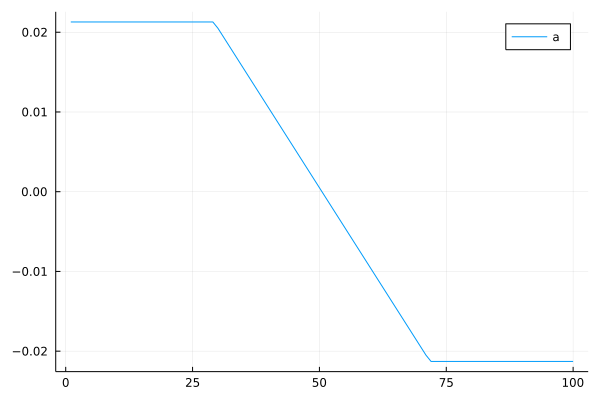
\includegraphics[width=\textwidth]{a.png}
        \caption{$a$}
    \end{subfigure}
    \hfill
    \begin{subfigure}[b]{0.3\textwidth}
        \centering
        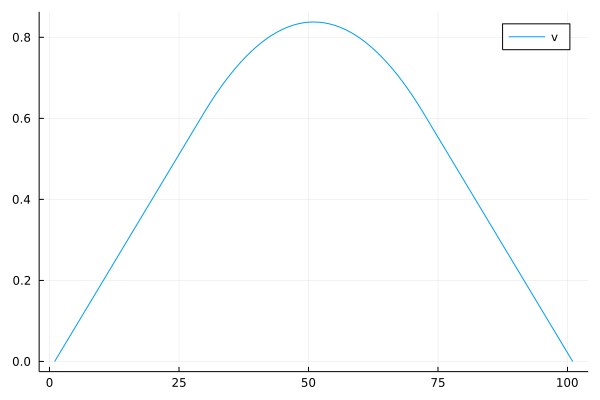
\includegraphics[width=\textwidth]{v.png}
        \caption{$v$}
    \end{subfigure}
    \hfill
    \begin{subfigure}[b]{0.3\textwidth}
        \centering
        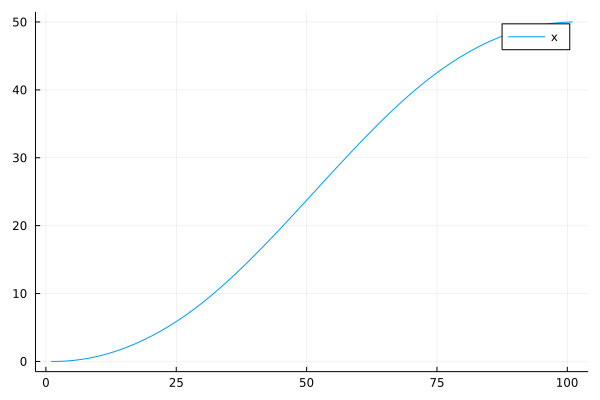
\includegraphics[width=\textwidth]{x.png}
        \caption{$x$}
    \end{subfigure}
       \caption{$a, x, v$ during the motion}
\end{figure}

\section{}

When $m\ge n$ this is trivial, so we consider $m < n$ only. For any $y\in\operatorname{ran}_+(A)$, consider the polyhedron

$$
C=\left\{x \in \mathbb{R}^{n} \mid y=A x, x \geq 0\right\}
$$

Assuming the rank of $A$ is $r\le m<n$, we can always select $r$ linearly independent rows such that, by row operations, they can eliminate other rows (including the corresponding elements in $y$). Therefore it suffices to prove the case $r=m$.

According to the corollary in class, every nonempty polyhedron in standard form has a BFS. $C$ is certainly nonempty since $y\in\textrm{ran}_+(A)$, so there exists a group of indices $B(1), \cdots, B(m)$ such that the matrix $B=(A_{B(1)}, \cdots, A_{B(m)})$ satisfies $B^{-1}y\ge 0$. This group of indices are the indices of coefficients required by the problem.

\section{}

\subsection{}

For (a), we noticed that $\bar c_2<0$, therefore $\beta=0$ (or else it can be further optimized). We choose $(\alpha,\beta,\gamma,\delta,\eta)=(0, 0, 0, 0, 0)$.

\subsection{}

For (b), we need $d_j>0,\forall j\in N$, so we choose $j=1$ and $\alpha,\gamma,\delta <0$. We choose $(\alpha,\beta,\gamma,\delta,\eta)=(-1, 0, -1, -1, 0)$.

\subsection{}

For (c), we choose $j=2$ to be optimized, so we require $\beta>0$. We choose $(\alpha,\beta,\gamma,\delta,\eta)=(0, 3, 0, 1, 0)$.

\end{document}